\documentclass[9pt,shortpaper,twoside,web]{ieeecolor}
\usepackage{generic}
\usepackage{cite}
\usepackage{amsmath,amssymb,amsfonts}
\usepackage{algorithmic}
\usepackage{graphicx}
\usepackage{textcomp}
\usepackage[utf8]{inputenc}
\usepackage[T1]{fontenc}
\usepackage{multirow}

\def\BibTeX{{\rm B\kern-.05em{\sc i\kern-.025em b}\kern-.08em
    T\kern-.1667em\lower.7ex\hbox{E}\kern-.125emX}}
\markboth{\journalname, Cercetare științifică 3}
{Author \MakeLowercase{\textit{et al.}}: O scurtă prezentare a metodelor de detectare a emoţiilor din semnalul vocal (Mai 2018) }

\begin{document}
\title{Keystroke Dynamics}
\author{Laurențiu-Iulian Iordache-Stoicescu }

\maketitle


\begin{abstract}
În ziua de astăzi, calculatoarele sunt folosite peste tot pentru a stoca și procesa o gamă largă de date. De asemenea, numărul atacurilor cibernetice a crescut și el. Pentru a putea proteja aceste sisteme de intruși, utilizarea unui sistem de securitate adecvat reprezintă o prioritate. În prezent sunt utilizate cu succes mai multe metode de securitate bazate pe măsuri biometrice, cum ar fi analiza amprentelor sau recunoașterea facială. Această cercetare se va axa însă pe o metodă prea puțin folită și anume, dinamica apăsării tastelor, cunoscută în literatură drept „Keystroke dynamics”.
\end{abstract}

\begin{IEEEkeywords}
SAAS - Software as a service;
PP - Press to press; 
RR - Release to release; 
RP - Release to press;
wpm - words per minuteș
\end{IEEEkeywords}


\section{Introducere}
\label{sec:introduction}


\subsection{Necesitate}
	Calculatoarele au devenit omniprezente în societatea modernă, conform statisticilor oferite de Internet World Stats \cite{b1}, numărul utilizatorilor unici de internet calculat la sfârșitul lunii Iunie 2018 este de aproximativ 4.2 miliarde. Pe cât este de mare numărul de utilizatori ce au acces la internet, pe atât de mare este numărul de atacuri cibernetice ce îi vizează. Conform datelor oferite de ..., aproximativ 63\% din toate intruziunile în rețele și furturile de informații se datorează compromiterii datelor de autentificare. Un atac cibernetic cunoscut care a constat în furtul datelor personale ale aproximativ 500 de milioane de conturi este cel ce a vizat site-ul „yahoo.com”.

	Din moment ce depindem din ce în ce mai mult de calculatoare, iar riscurile folosirii acestora cresc de la o zi la alta, este normal ca și nivelul de securitate să fie sporit pentru a putea face față atacurilor. Utilizarea de metrici biometrice în procesuld de autentificare este unul dintre pașii făcuți pentru sporirea securității în ceea ce privește autentificare unui utilizator. În acest caz se merge pe ideea că un atacator poate fura identitatea digitală a unui utilizator (utilizator, parola, token etc.) dar nu poate fura sau replica ceea ce este utilizatorul.

	În prezent sunt implementate cu succes mai multe metode de autentificare pe baza de metrici biometrice cum ar fi recunoașterea utilizatorului pe bază de amprentă papilară, recunoașterea facială sau a irisului. Aceste metode însă necesită componente hardware suplimentare pentru achiziția datelor biometrice. O altă metodă de identificare a unui utilziator, mai putin populară, o reprezintă analzia dinamicii apăsării tasterlor. Această metodă are avantajul că nu necesită componente hardware adiționale, deoarece orice calculator are o tastatură. Pe lângă acesta mai are un avantaj semnificativ și anume că poate realiza achiziția metricilor în timp ce utilizatorul își îndeplinește sarcinile uzuale fără a-l deranja și fără a se face sesizată achiziția de date, aceasta fiind o metodă neintruzivă.


\subsection{Generalități biometrie}


\subsection{Dinamica apăsării tastelor}
	Măsura biometrică a tastării este referită în literatură sub forma de „Keystroke dynamics” (dinamica apăsării tastelor). Dinamica apăsării tastelor se referă la felul în care o persoană apasă tastele unei tastaturi. Această metodă este bazată pe caracteristicile de scriere ale persoanelor cum ar fi durata apăsării unei taste, latența dintre apăsări consecutive ale tastelor, timpul dintre două apăsări consecutive și în cazul în care se poate, forța apăsării. Cele mai folositoare metrici sunt: timpul de apăsare, acesta reprezintă durata de timp a menținerii unei taste apăsate și timpul de pauză, care reprezintă durata de timp dintre eliberarea unei chei și apăsarea alteia.


\subsubsection{Istorie}	
	Această metodă este derivată din ideea de indentificare a expeditorului unui cod Morse ce folosește un telegraf. Această tehnică a fost analizată în timpul celui de-al doilea război mondial și poartă numele de „fist of the sender” (pumnul expeditorului). Aceasta a fost utilizată cu succes pentru a monitoriza deplasarea trupelor pe baza recunoașterii tiparului de transmisie a expeditorului mesajului \cite{b2}.

\subsubsection{Mecanismul psihologic}
	Avantajul utilizării de măsuri biometrice comportamentale cum ar fi dinamica apăsării tastelor îl reprezintă faptul că acestea pot fi colecate fără ca utilizatorul în cauză să își dea seama. 
	
	Experimentele psihologice efectuate în ultimul secol au demostrat că sarcinile repetitive cum ar fi vorbitul, scrisul, tastarea, cântatul la pian etc. sunt controlate de un set de acțiuni. Aceste acțiuni pot fi prezise folosind un model care descrie seria de pași efectuați pentru a realiza o sarcină \cite{b3}. Sistemul motor planifică planifică și controlează mișcarea pe baza informațiilor primite ca stimuli. Acesta poate fi privit ca pe un caz special de sistem auto-organizat \cite{4}. Pe parcursul secolului 20, s-au efectuat studii pentru ințelegerea fiziologiei și psihologiei deprinderilor sistemului motor. Studiile s-au axat asupra transmiterilor telegrafice. Studiile s-au efectuat pe 32 de subiecți cu nivel variat al deprinderii de telegrafiere. S-a observat că operatorii erau capabili să îi recunoască pe ceilalți operatori cu care au mai lucrat dor prin ascultarea caracteristicii de tastare, de asemenea, mulți dintre aceștia au susținut că erau capabili să determine și sexul operatorului \cite{b3}. 
	
\begin{figure}[htb]
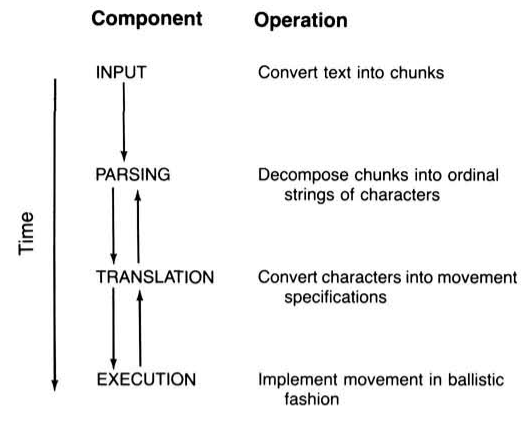
\includegraphics[width=0.9\columnwidth]{res/fig/modelul-cooper}
\caption{ \cite{b5}}
\label{fig1}
\end{figure}

	În figura 1 se poate observa modelul propus de W. E. Cooper, acesta reprezintă primul model general de tranzit al informației primite de un dactilograf, fiind împărțit pe etape pornind de la citirea textului până la transpunerea acestuia prin intermediul tastaturii. Prima etapă o reprezintă recunoașterea caracterelor. În această etapă s-a observat că dactilograful tinde să analizeze în avans materialul pe care îl scrie.


	A doua etapă constă în analizarea informațiilor citite. În această etapă, informațiile citite sunt stocate în memorie pentru o perioadă scurtă înainte de a fi scrise de mână. Conversia textului citit în acțiunea de tastare constă într-o combinație de procesări seriale și paralele ale informației. S-a observat că dactilografii împart textul în grupuri mici și predictibile datorită limitării memoriei \cite{b6}.

	A treia etapă o reprezintă translația caracterelor discrete în comenzi. Aceasta cuprinde acțiunea musculară efectuată pentru a executa mișcarea corectă a mâinii și a degetelor. S-a observat că succesiunea acțiunilor de mișcare a dactilografilor supuși experimentului este organizată înainte ca aceasta să fie executată și că aceasta este puternic influențată de starea actuală a subiectului. 
	
	A patra etapă constă în execuția efectivă a tastării urmată de un răspuns. În urma tastării, este oferit un răspuns vizual auditiv sau tactil. S-a observat și analizat semi-autonomia mișcării degetelor, aceasta fiind o acțiune care odata inițiată, nu mai poate fi oprită, ritmul și caracteristicile acesteia neputând fi falsificate. 



\section{Achiziția datelor}
	Pentru achiziția datelor se pot utiliza mai multe dispozitive cum ar fi: tastatura clasică utilizată pentru scriere, un tip special de tastatură care poate înregistra presiunea apăsării (deși această presiune poate fi aproximată pe baza timpului în care o tastă este apăsată), sau utilizarea unui ecran cu touchscreen, în cazul dispozitivelor mobile. Pe parcursul procesului de înrolare în sistem vor fi salvate diverse măsuri de timp precum și fraza unică tastată de utilizator (parola). După înrolarea acestuia, utilizatorul se va putea autentifica folosind parola și alți identificatori. Această informație va fi comparată de sistem cu parola existentă ca în cazul unui sistem clasic de autentificare dar se va verifica să coincidă și modul în care acesta a scris parola.
	
	
\subsection{Introducerea textului}
	Analiza dinamicii apăsării tastelor poate fi clasificată pe larg în două tipuri în funcție de tipul textului introdus - analiză a textului static sau structurat și analiza textului liber. 
	
	Analiza textului static implică analiza comportamentului de tastare a unui individ pentru fraze predeterminate într-un interval de timp bine definit. De exemplu, se poate considera analiza statică în momentul autentificării unui utilizator în sistem pe baza analizei dinamicii tastării id-ului și a parolei acestuia. Dar se mai  poate și analiza unei fraze particulare care este comună pentru fiecare utilizator al sistemului. Utilizarea analize textului static se folosește în mod normal în sistemele în care odată autentificat, nu mai sunt necesare introduceri suplimentare de date de la tastatură. Un exemplu de astfel de sistem îl reprezintă sistemul de autentificare într-un cont bancar. După autentificare, utilizatorul poate să citească datele tranzațiilor, să transfere sume etc.

	Analiza textului liber sau dinamic implică o analiză continuă periodică a comportamentului de tastare. Analiza are loc inițial la autentificarea în sistem și mai are loc pe parcursul utilizării acestuia. De exemplu, se poate utiliza un sistem de analiză a textului liber pentru a garanta dacă un anumit cont sau licență este folosit de mai mult de o persoană. Această metodă având mai multă aplicabilitate în aplicații de tip SAAS - Software as a service. Datorită naturii intruzive a acestei metode pot apărea probleme de intimitate. Pentru a evita astfel de probleme, în literatură a fost propusă utilizarea combinațiilor de patru taste consecutive stocate în matrici în loc de logare integrală a informației tastate.


\subsection{Mediul de achiziție}
	Mediul de achiziție joacă un rol important în determinarea caracteristicilor de scriere alea unui subiect. Mediul poate fi clasificat pe larg în două tipuri - mediu controlat și modiu necontrolat.

	S-au efectuat mai multe experimente pentru analiza comportamentului de scriere al utilizatorilor, pentru acestea s-a utilizat același sistem pentru fiecare utilizator într-un mediu cu o luminozitate și temperatură controlată. Un astfel de mediu este cunoscut ca mediu controlat. De asemenea pentru a se asigura că toți utilizatorii sunt acomodați cu tipul de tastatură utilizat, au fost lăsați să exerseze pe aceasta. Datele astfel colecate pot să nu fie relevante pentru condițiile actuale în care un utilizator scrie.
	
	Un mediu necontrolat poate fi definit ca un mediu în care sunt cunoscute parțial sau deloc caracteristicile acestuia. În astfel de medii, subiecților li s-a cerut esă realizeze achiziția datelor fie pe calculatoarele personale sau să completeze un formular online. Este preferată analiza și testarea sistemelor în medii necontrolate pentru perfecționare, chiar dacă cest date sunt mai greu de analizat datorită numărului mare de variabile ce pot interveni. Astfel se poate obține un sistem robust care să fie folosit de utilizatorul normal în propriul mediu.
	
	
\subsection{Caracteristici}
	În timpul scrierii, calculatorul poate înregistra tasta apăsată și timpul la care a fost apăsată, de asemenea, mai poate înregistra și timpul la care aceasta a fost eliberată și perioada de timp cât a fost apăsată, aceasta reprezentând diferența dintre primele două. În figura 2 sunt prezentate aceste informații temporale. Toate aceste informații pot fi stocate în timp ce un utilizator tastează.
	
\begin{figure}[htb]
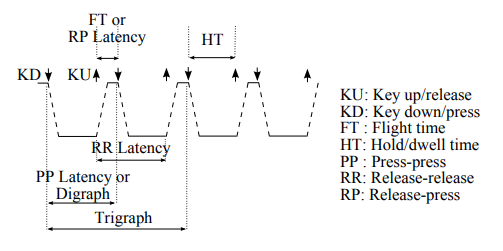
\includegraphics[width=0.9\columnwidth]{res/fig/keystroke-timing-information}
\caption{ \cite{b3}}
\label{fig2}
\end{figure}

	Latența reprezintă una dintre cele mai folosite caracteristici. Există trei astfel de latențe definite [9] - „press-to-press” PP(latența dintre două apăsări consecutive), „release-to-release” RR(latența dintre două eliberări consecutive), „release-to-press” RP (latența dintre o eliberare și o apăsare consecutive). Acestea trei mai sunt referite în literatură și sub alte nume, de exemplu, timpul dintre două apăsări consecutive mai este întâlnit sub forma de digraf, perioada de timp dintre eliberarea unei taste și apăsarea alteia se mai numește și „flight-time” (FT) (timp de zbod). S-a observat că este mai importantă latența de apăsare decât decât latența dintre apăsarea a două taste succesive \cite{b3}. 
		
	Pe baza acestor latențe se pot compune alte caracteristici, cum ar fi trigraful care reprezintă durata de timp necesară apăsării a trei taste consecutive, N-graful care reprezintă durata de timp necesară apăsării a N taste consecutive. S-a observat că utilizarea trigrafurilor oferă rezultate mai bune de clasificare decât în cazul utilizarii digrafurilor sau a N-grafurilor. 
		
	Pe lângă caracteristicile de timp, mai pot fi extrase și caracteristici de presiune. Acestea sunt extrase cu ajutorul unor tastaturi speciale ce permit măsurarea presiunii exercitate de utilizator la apăsarea unei taste. Aceste metrici au fost utilizate în încercarea a analizare a emoțiilor utilizatorului.

	Alte caracteristici secundare care pot fi derivate din caracteristicile de timp sunt viteza de scriere, aceasta este măsurată în cuvinte pe minut (wpm), viteza maximă/minimă, media și deviația standard a caracteristicelor și entropia.
	

\subsection{Metrici de performanță}
	În procesul de autentificare/verificare, se extrag datele din șirul de caractere introdus de utilizator pentru a crea un model al modului de tastare. Acest model este apoi comparat cu unul existent pentru utilizatorul respectiv, creat în momentul înrolării în sistem. Pentru comparare se folosește un algoritm care determină cât este de similar modelul nou creat cu cel existent în baza de date. Pentru procesul de identificare, verificarea este un proces de tip one-to-many, acesta constă în compararea modelului nou creat cu toate modelele din baza de date pentru a identifica utilizatorul.
	
	Pentru determinarea unui sistem biometric de autentificare utilizează două rate de eroare importante
- Rata de respingere falsă ,FRR („False Rejection Rate”) și rata de acceptare falsă, Far („False Acceptance Rate”). Acestea sunt reprezentate de următoarele rapoarte:


FRR reprezintă probabilitatea ca un sistem biometric să nu recunoască identitatea unui utilizator autorizat. Se definește ca fiind raportul dintre numărul de respingeri false și numărul total de încercări legitime de identificare a unui utilizator autentificat \cite{b7}.

\begin{equation} \label{eq2}
FRR = \frac{f_n}{t_p + f_n}
\end{equation}

FAR reprezintă probabilitatea ca un sistem biometric să confirme în mod eronat identitatea unui utilizator neautorizat. Se definește ca fiind raportul dintre numărul de acceptări false și numărul total de încercări de identificare a unui impostor \cite{b7}.

\begin{equation} \label{eq1}
FAR = \frac{f_p}{t_n + f_p}
\end{equation}

Unde: $f_n$ - numărul de respingeri false; $f_p$ - numărul de acceptări false; $t_n$ - numărul de respingeri corecte; $t_p$ - numărul de acceptări corecte.

	Se mai utilizează și măsura EER „Equal Error Rate” care reprezintă punctul de intersecție al curbelor trasate pentru FAR și FRR. Cu alte cuvinte $ERR = FAR = FRR$. Aceasta este utilizată pe post de indicator al preciziei sistemului biometric.
	
	Uzual, pentru sisteme biometrice în care securitatea nu este o prioritate, se permit valori mai mari ale FAR-ului însă în aplicații cu un nivel ridicat de securitate se preferă valori ridicate ale FRR-ului dar foarte scăzute lare FAR-ului. Cu cât este mai scăzută valoarea ERR-ului, cu atât sistemul biometric este mai precis.

\subsection{Baza de date}
% Enumerarea unor baze de date ce au fost achiziționate în medii controlate și în medii necontrolate.
	Lipsa de standardizare a achiziției datelor reprezintă pentru acest tip de măsură biometică un impediment în dezvoltare. Adoptarea de standarde ar trebui să faciliteze schimbul de informații între cercetători  și să ofere o mai bună metodă de comparare a diferiților algoritmi. Astfel se va reduce cu siguranță duplicarea efortului depus.
	În tabelul 1 sunt listate o parte din bazele de date făcute disponibile de anumiți cercetători. 
	
// TODO: De listat toate bazele de date în tabel și de discutat pe marginea lor.

\section{Abordări și rezultate}
	Odată extrase caracteristicile și create modelele, clasificarea utilizatorilor este realizată pe baza asemănărilor și deosebirilor dintre aceste modele. În literatură s-au utilizat de la metode simple derivate din statistică cum ar fi media și deviația standard provenite din statisica până la metode complexe de recunoaștere a acestora pentru clasificarea scriitorului. Algoritmii de clasificare s-au împărțit în patru categorii \cite{b7}.

\subsection{Algoritmi statistici}
	Cea mai simplă metodă statistică constă în calcularea mediei și deviației standard ale caracteristicilor modelului. Acestea pot fi folosite pentru compararea utilizatorilor folosind diverse modalități de testare cum ar fi: testarea ipotezei, t-tests și folosirea distanțelor cum ar fi distanța absolută, distanța Euclideană și a altor tipuri. În tamelul 2 pot fi vizualizate diverse abordări cu rezultatele acestora.
\\
\\

\begin{table}
	\begin{tabular}[c]{lcccccccc}
	\hline
	\multirow{2}{*}{Clasificare} & \multirow{2}{*}{TT} & \multirow{2}{*}{Env} & \multirow{2}{*}{S} & \multirow{2}{*}{M} & \multicolumn{3}{c}{Error rate (\%)} \\
	\cline{6-8}
            &    &     &   &   &  FAR & FRR & EER \\
	\hline
	Distanță abs. & S & C & 33 & 975 & 0.25 & 16.67 & - \\
	Distanță min. & S & C & 39 & 171 & 2.8  &  8.1  & - \\
	Distanță      & D & U & 30 &  -  & 8.33 &  3.33 & - \\
	Statistică    & D & C & 30 & 60  &15    &  0    & - \\
	Statistică    & S & C & 44 &220  & 0    &  2.3  & - \\
	Statistică    & S & C & 30 &553  & 1.89 &  1.45 & - \\
	\hline
	\end{tabular}
	
\caption*{
  A legend, even a table can be used
  \begin{tabular}{l l}
    item 1 & explanation 1 \\
  \end{tabular}
  }
\end{table}


\begin{thebibliography}{00}

\bibitem{b1} https://www.internetworldstats.com/stats.htm

\bibitem{b2} L. F. Coppenrath and Associates. „Biopassword Technology Overview”, http://www.lfca.net/Reference\%20Documents/Biometric\%20Solutions\%20By\%20Classification.pdf

\bibitem{b3} Salil P. Banerjee, Damon L. Woodard: „ Biometric Authentication and Identification using Keystroke Dynamics: A Survey”

\bibitem{b4} L. Shaffer. Tutorials in Motor Neuroscience, chapter Cognition and Motor Programming.
Kluwer Academic Publishers, 1991.

\bibitem{b5} T. A. Salthouse. Perceptual, Cognitive, and Motoric Aspects of Transcription Typing. Psychological Bulletin, 99(3):303 – 319, 1986.

\bibitem{b6} K. S. Balagani, V. V. Phoha, A. Ray, and S. Phoha. On the Discriminability of Keystroke Feature Vectors Used in Fixed Text Keystroke Authentication. Pattern Recognition Letters, 32:10701080, 2011.

\bibitem{b7} TODO: TBRSD - Curs de adăugat ref
\end{thebibliography}
\end{document}
